\documentclass{article}


% if you need to pass options to natbib, use, e.g.:
%     \PassOptionsToPackage{numbers, compress}{natbib}
% before loading neurips_2024

% submissions should not be anonymous, so use the 
% [preprint] option:
\usepackage[preprint]{paper}


% to avoid loading the natbib package, add option nonatbib:
%    \usepackage[nonatbib,preprint]{neurips_2024}


\usepackage[utf8]{inputenc} % allow utf-8 input
\usepackage[T1]{fontenc}    % use 8-bit T1 fonts
\usepackage{hyperref}       % hyperlinks
\usepackage{url}            % simple URL typesetting
\usepackage{booktabs}       % professional-quality tables
\usepackage{amsfonts}       % blackboard math symbols
\usepackage{nicefrac}       % compact symbols for 1/2, etc.
\usepackage{microtype}      % microtypography
\usepackage{xcolor}         % colors
\usepackage{geometry}
\usepackage{longtable}
\usepackage{graphicx}
\usepackage{amsmath}
\usepackage{booktabs}
\usepackage{caption}

\title{Smart Model Elimination for Efficient Automated Machine Learning in Healthcare}


% The \author macro works with any number of authors. There are two commands
% used to separate the names and addresses of multiple authors: \And and \AND.
%
% Using \And between authors leaves it to LaTeX to determine where to break the
% lines. Using \AND forces a line break at that point. So, if LaTeX puts 3 of 4
% authors names on the first line, and the last on the second line, try using
% \AND instead of \And before the third author name.


\author{%
  Eric Su Zhang$^1$ \\
  St. Mark's School of Texas\\
  10600 Preston Rd, Dallas, TX 75230\\
  \texttt{ericspring08@gmail.com} \\
  % examples of more authors
  \And
  Benjamin Joseph Michael Standefer$^2$ \\
  St. Mark's School of Texas \\
  10600 Preston Rd, Dallas, TX 75230 \\
  \texttt{bjmstandefer@gmail.com} \\
  % \AND
  % Coauthor \\
  % Affiliation \\
  % Address \\
  % \texttt{email} \\
  % \And
  % Coauthor \\
  % Affiliation \\
  % Address \\
  % \texttt{email} \\
  % \And
  % Coauthor \\
  % Affiliation \\
  % Address \\
  % \texttt{email} \\
}


\begin{document}


\maketitle


\begin{abstract}
  Automated Machine Learning or AutoML has emerged as a popular field of research. We performed a literature review of existing AutoML papers and conducted an in-depth survey on five popluar AutoML frameworks. Many of these frameworks optimize a form of model selection, however, they all require every model to be run and evaluated. We propose a novel framework, SMEML (Smart Model Elimination Machine Learning), that automatically eliminates models that are unlikely to be performant. SMEML demonstrates the ability to generate a model with near equal accuracy to a "dumb" brute-force model, but in a fraction of the time. We also believe this innovation is particularly relevant to machine learning in healthcare because of the necessity for efficient diesease prediction. 
\end{abstract}


\section{Introduction}

Machine learning (ML) is a type of artificial intelligence (AI) that uses searching and trend-determining to make predictions. ML algorithms are trained and tested on a given dataset to become "smarter". Once they've learned the patterns typical of that data, they can make predictions based on similar but unseen data. These algorithms also require additional processes, however, like hyperparamater tuning, and can be modified in conjunction with one another, like in ensemble learning. This makes the process complex and time-inefficient. To do this on a larger scale and at greater speeds, recent research and effort have been put into Auto ML frameworks [1].

One sector of the global industry that has the most potential for beneficial integration of AutoML frameworks is healthcare, particularly in developing countries. These countries have severe shortages of healthcare workers and limited tools for diagnosis. For example, Africa has 2.3 healthcare workers per 1000 individuals, while the Americas have 24.8 healthcare workers per 1000 [2]. The World Health Organization (WHO) emphasized that this deficit is growing every year and will likely reach 18 million personnel by 2030 [3]. Medical AI's typically automate repetitive tasks, making time consumption a primary concern [4]. This coupled with a lack of adequate resources makes designing faster diagnostic systems for developing countries' medical sectors a pivotal issue. 
%
Most AutoML frameworks implement some form of model selection where a pool of models are filtered until a final model is selected. However, these frameworks require that every model to be run to filter out [1]. In theory, this means that much energy is spent training models that are unlikely to be selected. We propose SMEML, a novel model selection algorithm that automatically eliminates models that it believes will not be performant. 

\subsection{Survey}

\begin{table}
  \caption{Survey of Existing AutoML Frameworks}
  \label{automl-survey}
  \centering
  \begin{tabular}{lllllllll}
    \toprule
    Framework & EOU & M & FE & TM & HPT & Inter & Custom\\
    \midrule
    H2O AutoML & Easy & 12 & Basic & Yes & Auto & SHAP & High\\
    TPOT & Hard & 10 & Basic & No & Genetic & POJO & Moderate\\
    MLJAR & Easy & 12 & Advanced & Yes & Auto & Basic & High\\
    FLAML & Easy & 9 & Limited & Yes & Auto & SHAP & Low-Moderate\\
    LightAutoML & Easy & 11 & Advanced & Yes & Auto & Basic & Moderate\\
    \bottomrule
  \end{tabular}
  \captionsetup{font=footnotesize}
  \caption*{\textbf{Abbreviations}: EOU: Ease of Use, M: \# of models evaluated by framework, FE: Feature Engineering, TM: Time Management, HPT: Hyper-Parameter Tuning, Inter: Interface, Custom: Customization}
\end{table}
We systematically reviewed and compared five different AutoML frameworks, comparing every feature relevant to medical implementation [5-10]. Of these six, we wanted to take a closer look at four: FLAML, H2O, MLJAR, and TPOT.

We can observe pros and cons in the four models' theoretical applications. FLAML uses blend search hyper-parameter optimization and focuses on lightweight models, making it quick and applicable to repetitive tasks. It supports user-specified imputation techniques for missing values and has an intuitive API, making it moderately user-friendly for healthcare workers [9]. H2O has a wider variety of supported algorithms that may be appropriate for medical diagnosis, making it slower than FLAML on average. In one trial, more than half of FLAML's performances in one minute were better than or equal to H20's performances in one hour [9]. H2O has automatic and multi-faceted methods of dealing with missing values and flexible interfaces in R and Python, making it intuitive for users [5]. MLJAR uses advanced algorithms such as light gradient boosting and neural networks. It automatically deals with missing values and is known for its automated user interface [7]. TPOT uses genetic programming. It builds pipelines over multiple generations, which can be time consuming. It has built-in pre-processing for missing values, but the genetic programming can require fine-tuning from users [6].

Keeping the factors we have laid out in mind, namely expeditious running, accuracy, and interpretability, we also uncovered a key continuity in framework design: frameworks are forced to run and train the majority of their available models to maximize accuracy at the expense of efficiency. Given the restricted nature of tabular data, there are some models that are less likely to perform well, thus running and training these models is frequently wasteful. Cutting these models completely, however, is not optimal either, as they are the best option in a minority of cases. We hypothesized that using a combination of layered machine learning implementation and meta-feature extraction would yield an equally versatile system that minimizes time spent on prediction while still maximizing the other quantities. 

\section{Methodology}
When considering a specific dataset, various aspects regarding the distribution and relationship within the data can give us clues as to which models are likely to perform best. For example, linear models tend to work better on datasets where there is a linear relationship between features [11]. As a result, we can develop a boosting model to predict the best models based off extracted attributes from a dataset. These extracted attributes are shown in Table 2. Each attribute attempts to capture a specific type of relationship or distribution within the data. The variable importance of each attribute is shown in the "Weight" column. Linearity and data distribution are the most important attributes in determining the best model.

We considered 28 different models, including all supervised and semi-supervised sklearn classification models and common boosting models such as XGBoost, Lightgbm, and Catboost.

To implement this model elimination process, we trained a boosting model on 268 kaggle datasets. We chose datasets that were medically related and focused our approach on binary classification. We extracted the attributes in Table 2 from each dataset: this is the input for the boosting model. We then ran a "dumb" framework that trained every model on each dataset. The accuracy of every model is ranked and every model is treated as a label with its value being its rank. Then we trained a multilabel regression to predict the rank of each model, giving the extracted attributes. We produced a median spearman correlation of 0.7301 between the predicted rank and the actual rank and a median p-value of 1.032e-05. Furthermore, we guarantee that we can predict a top two model within the predicted top eight 90.12\% of the time.

When a user inputs a dataset into SMEML, it first extracts the attributes from the dataset. It feeds these attributes into the boosting model to get the predicted rank of each model. Since we have determined that we can predict a top two model within the predicted top eight quite confidently, we can eliminate the bottom 18 models from the list. We run Bayseian optimization on the top eight models to get the best hyperparamters for each model. We select the top models that have significantly better performance than other models. These models are stacked together to form the final model. This process is shown in Figure 1.
\begin{table}
  \caption{Attributes extracted from a dataset}
  \label{model-options-table}
  \centering
  \begin{tabular}{llll}
    \toprule
    Attribute & Formula & Purpose & Weight\\
    \midrule
    \# of Rows & $|\mathbf{A}|_r$ & DS & .0422 \\
    \hline
    \# of Columns & $|\mathbf{A}|_c$ & DS & .0415 \\
    \hline
    Target Distribution &
    $\frac{\max(\text{count}_1, \text{count}_0)}{|\mathbf{A}|_r}$
    & DT & .0489 \\
    \hline
    Numerical Columns &
    $\frac{|\mathbf{A}_{num}|}{|\mathbf{A}|_{c}}$
    & DT & .0428 \\
    \hline
    Binary Categorical Columns &
    $\frac{|\mathbf{A}_{bin}|}{|\mathbf{A}|_{c}}$
    & DT & .0117 \\
    \hline
    Mean \# of Distinct Values  & $\mu \left\{\text{\# of distinct values in column}\right\}$ & DT & .0076 \\ 
    \hline
    Mean IQR  & $\mu \left\{\text{IQR of column}\right\}$ & DD & .0594 \\ 
    \hline
    STD of IQR  & $\sigma \left\{\text{IQR of column}\right\}$ & DD & .0700 \\
    \hline
    Mean Q1 & $\mu \left\{\text{Q1 of column}\right\}$ & DD & .0789 \\
    \hline
    STD of Q1  & $\sigma \left\{\text{Q1 of column}\right\}$ & DD & .0613 \\
    \hline
    Mean Q3  & $\mu \left\{\text{Q3 of column}\right\}$ & DD & .0812 \\
    \hline
    STD of Q3  & $\sigma \left\{\text{Q3 of column}\right\}$ & DD & .1103 \\
    \hline
    Mean Percent of Z-Score Outliers  & 
    $\mu \left\{ \frac{\text{\# of Z-Score Outliers}}{|\mathbf{A}|_r} \right\}$ & ODP & .0558 \\
    \hline
    STD of Percent of Z-Score Outliers  &
    $\sigma \left\{ \frac{\text{\# of Z-Score Outliers}}{|\mathbf{A}|_r} \right\}$ & ODP & .0798 \\
    \hline
    Mean Correlation& $\mu \left\{\text{Correlation Matrix}\right\}$ & DL & .0559 \\
    \hline
    STD of Correlation & $\sigma \left\{\text{Correlation Matrix}\right\}$ & DL & .1526 \\
    \bottomrule
  \end{tabular}
  \captionsetup{font=footnotesize}
  \caption*{\textbf{Abbreviations}: DS: Data Size, DT: Data Type, DD: Data Distribution, ODP: Outlier Data Points, DL: Data Linearity}
\end{table}


\begin {figure}
\centering
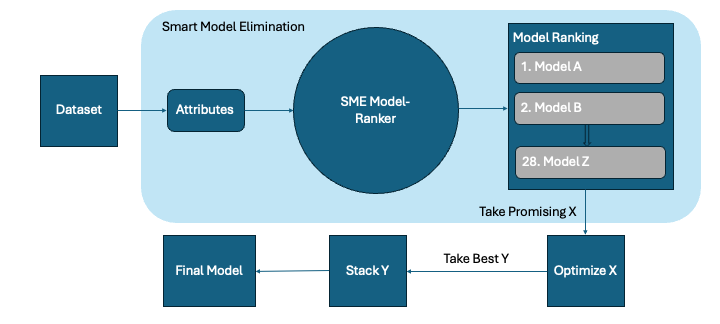
\includegraphics[width=\textwidth]{smeml-flowchart.png}
\caption{SMEML Process}
\end{figure}

\section{Experiments}
\subsection{Experiment Design}
To evaluate our framework, we choose 5 different datasets of diverse size. We ran SMEML on each dataset for 20 iterations of tuning. We compared this against a "dumb" mode which simply runs every model on the dataset. We used the accuracy and time to train as our metrics. All experiments are run on an Ubuntu server with Intel Xeon E5520 @ 2.27GHz and 24GB of RAM.

\subsection{Results}
\begin{table}
  \caption{Experiment Results}
  \label{model-options-table}
  \centering
  \begin{tabular}{llllll}
    \toprule
    % group 2, 3 as multicolumn and 4, 5 as multicolumn
    Dataset & \multicolumn{2}{c}{Accuracy} & \multicolumn{2}{c}{Time to Train (sec)} & Size (RxC)\\
    \cmidrule(lr){2-3} \cmidrule(lr){4-5}
    & SMEML & Dumb & SMEML & Dumb \\
    \midrule
    Lung Cancer Prediction [12] & .9839 & .9839 & 143.07 & 317.04 & 309x16\\
    Chronic Kidney Disease Dataset [13] & 1.0 & 1.0 & 419.64 & 788.46 & 400x26\\
    Pima Indians Diabetes Dataset [14] & .7857 & .8052 & 161.99 & 374.01 & 768x8 \\
    Brain Stroke Prediction Dataset [15] & .9458 & .9458 & 114.16 & 370.95 & 4892x11\\
    Stroke Prediction Dataset [16] & .9393 & .9393 & 172.67 & 385.23 & 5110x12 \\
    Eye State Classification [17] & .9536 & .9549 & 312.57 & 696.51 & 14980x15\\ 
    \bottomrule
  \end{tabular}
\end{table}

Several observations were readily apparent from running these datasets. First, accuracy did not change for 4 of the 6 benchmarks. The other two benchmarks on eye states and diabetes prediction represented a loss of accuracy for SMEML by 0.13\% and 1.95\%, respectively. Training time, however, favored SMEML in every trial. SMEML outperformed the dummy framework by 173.96 seconds in its worst performance on the lung cancer trial and by 383.94 seconds in its best performance on the eye state dataset. Relative to the dummy's performance, a percent decrease in time to run for SMEML of at least 46.78\% could be seen, with a decrease of up to 69.22\% observerd as well. SMEML's worst performance by percent decrease was also the performance in which it returned perfect accuracy. 
\section{Discussion}
\subsection{Summary}
SMEML manages to return comparable accuracy results compared to its dumb couterpart while more than splitting the run time in half in the majority of benchmarks. Its performance is not limited by the size of the dataset, and it in fact returned its first, third, and fourth best percentage-based run times on the 'large' dataset benchmarks (those exceeding 1000 rows). This is important in third world medicine where time is of the essence and there is a constant influx of new patient data. Further research should be done in incorporating this innovation into a full-fledged AutoML framework to expedite and improve the process further. A practical demonsration of this software's real-world application can be found on our SmartDx website [18]. Source code can be found at [19].
\subsection{Limitations}
Our implementation of SMEML has limitations. These include a small training set due to lack of available datasets, finite computing power, time constraints, and a lack of access to paticular scientific literature. Our framework only improves on the model selection process and does not address the various other aspects of AutoML. Therefore, SMEML is not comparable to other full-featured AutoML frameworks.
\subsection{Future Work}
Future work will include increasing the size of the training set, implementing a fully fledged AutoML framework, and conducting a detailed experiment comparing SMEML to other popular AutoML frameworks. Furthermore, we can examine other types of machine learning such as regression and multiclass-classification.
\begin{ack}
The authors would like to thank the St. Mark's School of Texas for supporting this research.
\end{ack}

\section*{References}

\medskip
{
\small

[1] He, Xin, et al. “AutoML: A Survey of the State-of-the-Art.” Knowledge-Based Systems, 212, 106622 (2021), \url{https://doi.org/10.1016/j.knosys.2020.106622}. 

[2] Nchasi, Goodluck, et al. “Challenges Faced by African Healthcare Workers During the Third Wave of the Pandemic.” Health Science Reports, 5, 6 (2022), \url{https://doi.org/10.1002%2Fhsr2.893}.

[3] Global Strategy on Human Resources for Health: Workforce 2030. World Health Organization, 16 (2016), \url{}.

[4] Bajwa, Junaid, et al. “Artificial Intelligence in Healthcare: Transforming the Practice of Medicine.” Future Healthcare Journal, 8, 188-94 (2021), \url{https://doi.org/10.7861%2Ffhj.2021-0095} 

[5] LeDell, E., and S. Poirier. “H2O AutoML: Scalable Automatic Machine Learning.” 7th ICML Workshop on Automated Machine Learning, 2020, \url{www.automl.org/wp-content/uploads/2020/07/AutoML_2020_paper_61.pdf}.

[6] Olson, Randal S., 1, et al. "Automating Biomedical Data Science Through Tree-based Pipeline Optimization." Applications of Evolutionary Computation, 19, 123 (2016), \url{https://doi.org/10.1007/978-3-319-31204-0_9}.

[7] P\l{}o\'{n}ska, Aleksandra, et al. “MLJAR: State-of-the-art Automated Machine Learning Framework for Tabular Data.  Version 0.10.3.” MLJAR, (2021), \url{github.com/mljar/mljar-supervised}.

[8] Conrad, Felix, et al. “Benchmarking AutoML for Regression Tasks on Small Tabular Data in Materials Design.” Scientific Reports, 12, 19350 (2022), \url{https://doi.org/10.1038/s41598-022-23327-1}.

[9] Shang, Zhi, et al. "FLAML: A Fast and Lightweight AutoML Library." 4th MLSys Conference, (2021), \url{https://doi.org/10.48550/arXiv.1911.04706} .

[10] Ryzhkov, Alexander, et al. "LightAutoML: AutoML Solution for a Large Financial Services Ecosystem." arXiv, (2021), \url{https://doi.org/10.48550/arXiv.2109.01528}

[11] Akalin, Altuna. 3.3 Relationship Between Variables: Linear Models and Correlation | Computational Genomics With R. 30 Sept. 2020, \url{compgenomr.github.io/book/relationship-between-variables-linear-models-and-correlation.html}.

[12] Ms. Nancy Al Aswad. Lung Cancer. \url{www.kaggle.com/datasets/nancyalaswad90/lung-cancer}.

[13] Mansoor Iqbal. Chronic KIdney Disease Dataset. \url{www.kaggle.com/datasets/mansoordaku/ckdisease}.

[14] UCI Machine Learning. Pima Indians Diabetes Dataset. \url{https://www.kaggle.com/datasets/uciml/pima-indians-diabetes-database}.

[15] Izzet Turkalp Akbasli. Brain stroke prediction dataset. \url{https://www.kaggle.com/datasets/zzettrkalpakbal/full-filled-brain-stroke-dataset}.

[16] fedesoriano. Stroke Prediction Dataset. \url{www.kaggle.com/fedesoriano/stroke-prediction-dataset}.

[17] Rob Mulla. Eye State Classification EEG Dataset. \url{https://www.kaggle.com/datasets/robikscube/eye-state-classification-eeg-dataset}.

[18] SmartDx Website. \url{https://smartdx.vercel.app/}.

[19] Github Repository. \url{www.github.com/ericspring08/SMEML-Paper}.
}

\end{document}
